\documentclass{article}


% if you need to pass options to natbib, use, e.g.:
%     \PassOptionsToPackage{numbers, compress}{natbib}
% before loading neurips_2023


% ready for submission
\usepackage[final]{neurips_2023}


% to compile a preprint version, e.g., for submission to arXiv, add add the
% [preprint] option:
%     \usepackage[preprint]{neurips_2023}


% to compile a camera-ready version, add the [final] option, e.g.:
%     \usepackage[final]{neurips_2023}


% to avoid loading the natbib package, add option nonatbib:
%    \usepackage[nonatbib]{neurips_2023}


\usepackage[utf8]{inputenc} % allow utf-8 input
\usepackage[T1]{fontenc}    % use 8-bit T1 fonts
\usepackage{hyperref}       % hyperlinks
\usepackage{url}            % simple URL typesetting
\usepackage{booktabs}       % professional-quality tables
\usepackage{amsfonts}       % blackboard math symbols
\usepackage{nicefrac}       % compact symbols for 1/2, etc.
\usepackage{microtype}      % microtypography
\usepackage{xcolor}         % colors
\usepackage{graphicx}
\graphicspath{ {./images/} }
\title{Examining if Linear regression is a good model for predicting Received RF Signal Strength with frequency and bandwidth as predictors.}


% The \author macro works with any number of authors. There are two commands
% used to separate the names and addresses of multiple authors: \And and \AND.
%
% Using \And between authors leaves it to LaTeX to determine where to break the
% lines. Using \AND forces a line break at that point. So, if LaTeX puts 3 of 4
% authors names on the first line, and the last on the second line, try using
% \AND instead of \And before the third author name.


\author{%
  Michael S.~Odom\thanks{Graduate Student.} \\
  CpE 590\\
  University of Alabama in Huntsville\\
  Huntsville, AL 35899 \\
  \texttt{mso0007@uah.edu} \\
  % examples of more authors
  % \And
  % Coauthor \\
  % Affiliation \\
  % Address \\
  % \texttt{email} \\
  % \AND
  % Coauthor \\
  % Affiliation \\
  % Address \\
  % \texttt{email} \\
  % \And
  % Coauthor \\
  % Affiliation \\
  % Address \\
  % \texttt{email} \\
  % \And
  % Coauthor \\
  % Affiliation \\
  % Address \\
  % \texttt{email} \\
}


\begin{document}


\maketitle


\begin{abstract}
  This paper will explore my findings on using Linear Regression to predict received signal strength, based on frequency and bandwidth. Overall, based on the results, this was found to be a poor prediction method, but may have been due to what data was found in the dataset.
\end{abstract}


\section{Background}


When analyzing an Radio Frequency(RF) communication channel, Signal-to-Noise (SNR) ratio is the figure of merit. SNR is calculated with a version of the \emph{Friis Transmission Equation} as follows: 

\[ SNR = \frac{Received Signal Strength}{NoisePower} 
$$

Where:

\[ Received Signal strength(Watts) =  Transmit Power(Watts) * Transmit Antenna Gain(Watts) * Receive Antenna Gain(Watts) * ( wavelength(m)/(4*Pi*distance(m)))^2$$ 

And:

\[ Noise Power = Boltzmann constant*temperature*Bandwidth$$

The dataset "RF Signal Data" by SURAJ on Kaggle was used to perform a linear regression regression. 

\subsection{RF Background}


A few notes on the nature of the data used. Signal Strength is presented in dBm, so Frequency and Bandwidth are translated from Hertz into Log space using this relationship:

\[ dBspace = 10*Log10(LinearValue)$$

The reason these values were chosen as predictors is due to Frequency's proportional relationship to signal strength, as well as its relationship to wavelength:
\[ wavelength = \frac{SpeedofLight}{Frequency}$$

which as a squared term could be "overpowering.
Bandwidth was chosen as a predictor due to its quality of "Spreading the power."




\subsection{Linear Regression}

Linear Regression is a "kind of supervised machine learning algorithm where a linear discriminant model g(x) is used to fit on the Given DataSet."(Bhadani)

More Generally:

\[ g(X) = w^T*x +w_{0}$$


Where: $w^{T}$ is the weights transposed and $w_{0}$  is the bias.

This is commonly seen as the "easiest" Machine learning algorithm and as such one that is commonly used.


\subsection{Dataset}

The dataset was downloaded from Kaggle as a CSV. Due to the massive size of the file, I used the first 1300 rows to perform my analysis. 

To clean the data, I added two additional columns to translate Frequency and Bandwidth to "logspace."

The Dataset only contained one set of coordinates per entry sand the same location name, so an assumption was made that all the distances were equal.

Also worth noting is that the dataset lacked Transmit power data, which is a key parameter in link analysis.




\section{Results}
\label{gen_inst}

First I looked at the correlation between various features.

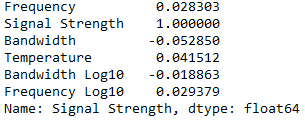
\includegraphics{Screenshot_corr}
 
And looked at graphically:

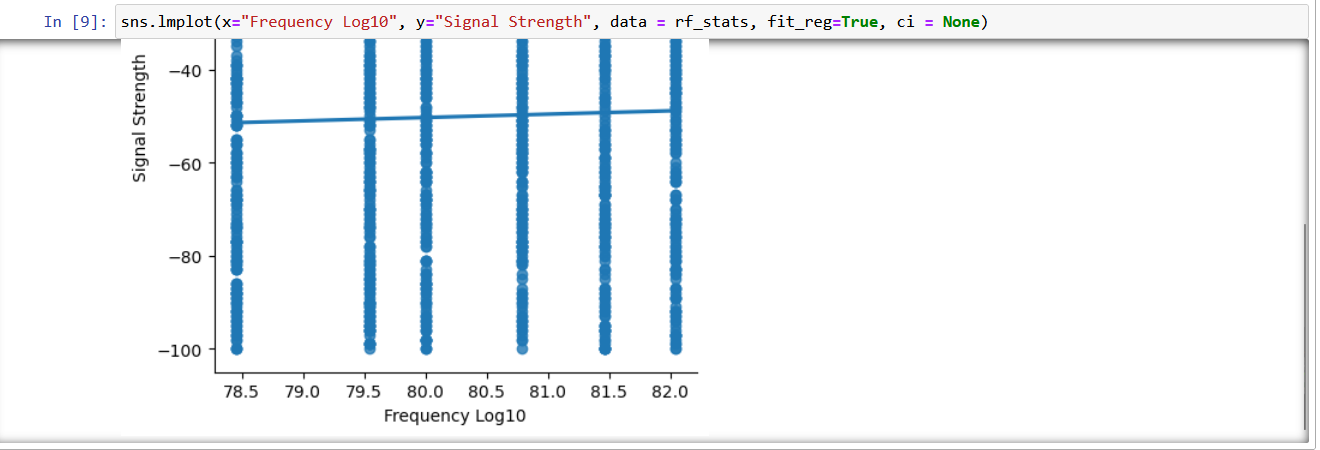
\includegraphics[width=100mm]{Screenshot_plot}

It seems there is an incredibly weak correlation, in fact here is the mean absolute error and statistics of the dataset:

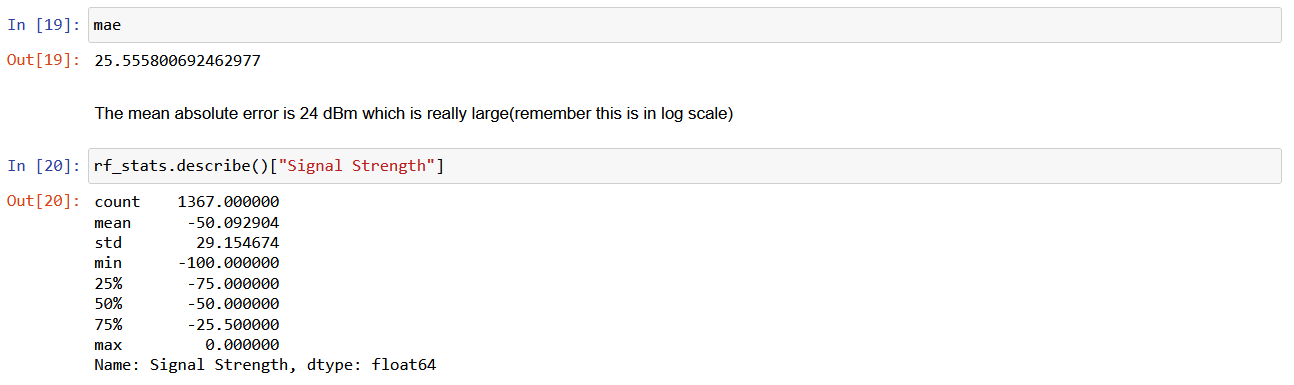
\includegraphics[width=100mm]{mae}

The Mean Absolute error is lower than the standard deviation, despite the correlation being relatively low when calculated.



\section{Conclusion}
\label{headings}

It seems that linear regression is a poor fit when using frequency and bandwidth as predictors. For further investigation into this topic, I plan to look for a data set containing transmit power and distance as features. Since distance is included as a term in receive signal strength that is squared, it is most like more overpowering as it grows larger. Likewise, transmit power and gain provide an upper limit on what the receive strength should be. This project has really exposed to me the importance (and difficulty!) of finding a quality dataset.


\section*{References}

{
\small


[1] Rahul Bhadani Assistant Professor Electrical and Computer Engineering The University of Alabama in Huntsville's notes




[2] The RF Signal Dataset found at: https://www.kaggle.com/datasets/suraj520/rf-signal-data?resource=download

}

%%%%%%%%%%%%%%%%%%%%%%%%%%%%%%%%%%%%%%%%%%%%%%%%%%%%%%%%%%%%


\end{document}